
%(BEGIN_QUESTION)
% Copyright 2006, Tony R. Kuphaldt, released under the Creative Commons Attribution License (v 1.0)
% This means you may do almost anything with this work of mine, so long as you give me proper credit

Two pressure-actuated ``lifts'' are used to raise a heavy weight off the ground.  One lift uses oil under pressure (from a hydraulic pump) while the other lift uses air under pressure (from an air compressor).  Each lift is equipped with a shut-off valve on the line feeding fluid to the cylinder, so that the piston's motion may be halted:

$$\includegraphics[width=15.5cm]{i00750x01.eps}$$

What will happen if the weight were to fall off the lift platform after it had been raised up from ground level, in each case?  Assume that the shut-off valve is closed (no fluid flow from pump or compressor into the cylinder) when this happens.

\vskip 20pt \vbox{\hrule \hbox{\strut \vrule{} {\bf Suggestions for Socratic discussion} \vrule} \hrule}

\begin{itemize}
\item{} What general lessons may we draw from this example regarding pressurized fluid safety?
\item{} Does the calculation of piston force based on pressure ($F = PA$) change at all if the fluid in question is a {\it gas} rather than a {\it liquid}?
\end{itemize}

\underbar{file i00750}
%(END_QUESTION)





%(BEGIN_ANSWER)

If the weight falls off the oil-actuated lift, the piston will hold its original position.  If the weight falls off the air-actuated lift, the piston will rise substantially (perhaps even ejecting from the cylinder!) due to expansion of the air:

$$\includegraphics[width=15.5cm]{i00750x02.eps}$$

%(END_ANSWER)





%(BEGIN_NOTES)

This question comes from an anecdote related to me by one of my former classmates in college: he was working as an air-conditioning duct installer, and was using an air-powered lift to hoist a large box of sheet metal and tools up to a rooftop.  As soon as he pulled the box off the lift platform, the platform and cylinder shot up, popping out of the cylinder completely, crashing in the alley below!  Fortunately, no one was hurt.

%INDEX% Mechanics, fluid power systems: hydraulic/pneumatic car lift
%INDEX% Physics, static fluids: compressibility

%(END_NOTES)


